\chapter{Estudo de caso: A.M.I.G.O.S.}
\label{ap:estudo}

Nosso estudo de caso aplica-se sobre um ambiente digital de interação
desenvolvido para a gestão do conhecimento em rede social. Durante o estudo de
caso aplicamos a metodologia proposta no \chapref{ch:kddm} e seu passo a passo
será descrito nas seções \ref{ap:sec:dominio}, \ref{ap:sec:dados},
\ref{ap:sec:preparacao} e \ref{ap:sec:analise}. Nos resultados avaliaremos a
utilidade do método e das ferramentas desenvolvidas no processo.

\section{Entendendo o domínio}
\label{ap:sec:dominio}

Nosso objetivo neste processo de mineração é analisar uma ``fotografia'' do
ambiente digital do a.m.i.g.o.s. e extrair dela um grupo de atores-chaves;
aqueles que se destacam dos demais pelo seu posicionamento ou influência sobre a 
rede. Para darmos prosseguimento a análise, precisamos entender o ambiente e
decidir sobre a ferramenta de análsie que usaremos. Sobre o ambiente temos:

\begin{quote}{\citep{RicardoAraujoCosta2008}}
	Acrônimo de Ambiente Multimídia para Integração de Grupos e Organizações Sociais,
	o a.m.i.g.o.s tem por objetivo prover a infra-estrutura necessária para a criação
	de redes sociais virtuais para os mais diversos fins. Dentre estes, pode-se
	destacar o seu uso para estimular a criação e compartilhamento do conhecimento
	pelos seus diversos membros, podendo estes estarem relacionados a uma organização
	social. Nele é permitida a criação explícita das redes sociais através dos
	usuários e seus contatos. Cada contato é explicitamente adicionado por cada
	usuário, mesmo que dentro de uma mesma organização, e este relacionamento é
	navegável por qualquer outro membro da rede social. Nas próximas linhas são
	apresentadas as principais funcionalidades com suas características e possíveis
	usos.
	\begin{description}
	\item[Perfis] Cada usuário possui um perfil no a.m.i.g.o.s. Este perfil
	consiste de um conjunto de dados preenchidos na forma de cadastro, que definem
	algumas propriedades simples do usuário, como local de residência, idiomas que
	possui conhecimento, endereço de e-mail, identificadores de aplicações de
	mensagem instantânea (Windows Live Messenger, Skype, Google Talk, dentre
	outros), e uma descrição de suas áreas de interesse. Porém a parte mais
	relevante do perfil não é preenchida pelo usuário, e sim inferida pelo
	sistema. [\emph{Para cada usuário, um índice de atividade para a produção e
	consumo de conteúdos também é automaticamente calculado}]
	\item[Histórias] Histórias são destinadas ao registro, compilação e
	apresentação de conhecimentos emergentes entre os participantes da rede.
	Construído de forma gradual, através de contribuições espontâneas ou
	induzidas, qualquer usuário do sistema pode inserir no ambiente suas próprias
	histórias de sucesso ou dilemas, à medida que as considere relevantes para o
	objetivo da rede social. Adicionalmente as histórias podem estar associadas a
	uma ou mais comunidades, o que indica que, apesar do autor ser um usuário em
	específico, o conhecimento construído encontra-se de alguma forma relacionado
	a estas comunidades.

	Cada usuário do sistema poderá, adicionalmente, atuar como um revisor do
	conteúdo inserido por seus pares, avaliando qualitativamente as contribuições
	disponibilizadas neste ambiente. Esta avaliação pode ser realizada de uma das
	duas formas:
	\begin{itemize}
	  \item Adição de comentários que contribuam para a evolução da história,
	  criando-se assim uma história mais rica, com mais participantes e novos
	  conhecimentos. À medida que a história for acrescida de comentários, é criado
	  um diálogo associado ao conhecimento em construção;
	  \item Atribuição de uma nota, variando de uma (1) a cinco (5) estrelas, às
	  histórias que lê. Permitindo que este conhecimento, expresso através de
	  histórias, possa ser apresentado através de um ranking que indique as mais
	  relevantes para os membros daquela rede social.
	\end{itemize}
	\item[Relacionamentos] O a.m.i.g.o.s dá suporte a praticamente todos os
	mecanismos de relacionamentos existentes nas atuais redes sociais. Nele cada
	usuário pode adicionar a sua lista de contatos qualquer outro usuário também
	membro da rede social. Esta lista de contatos pode ser agrupada em grupos,
	facilitando a organização dos contatos pelo seu usuário.
	\item[Comunidades Virtuais] Comunidades podem ser vistas como agregações de
	pessoas com objetivos em comum. O a.m.i.g.o.s dá suporte à criação de
	manutenção de comunidades por parte de seus usuários, podendo estes convidarem
	membros de sua lista de contatos a participar das discussões ou atividades a
	serem realizadas no âmbito da comunidade.

	Cada comunidade possui uma série de mecanismos para a criação e
	compartilhamento do conhecimento. O principal mecanismo de criação e
	compartilhamento do conhecimento é o fórum de discussão, onde os membros da
	comunidade podem iniciar discussões sobre os mais diversos assuntos.

	Um segundo mecanismo de compartilhamento do conhecimento é a associação de
	histórias à comunidade. Esta associação pode ser realizada por qualquer membro
	da comunidade ao criar uma história no sistema. Caso deseje-se, é possível até
	mesmo que a história seja visível apenas pelos membros das comunidades
	relacionadas.
	\item[Recomendações] Como mecanismo de disseminação do conhecimento, o
	a.m.i.g.o.s possui suporte a recomendações. Estas recomendações são sempre
	direcionadas a usuários do sistema e podem ser referentes a histórias,
	comunidades, tópicos de um fórum ou outros usuários. Existem basicamente dois
	tipos de recomendação, uma feita manualmente por um usuário para seus
	contatos, e a outra realizada automaticamente pelo sistema para um usuário a
	partir da probabilidade do interesse deste no conteúdo recomendado.

	Para que a recomendação automática seja possível, o sistema vai montando o
	perfil do usuário à medida que este utiliza o sistema, baseado no que é lido ou
	escrito por ele. Para isto, o sistema faz uso do \emph{Vector Space Model}
	\citep{Barros2002}, varrendo o conteúdo textual disponível em cada elemento,
	calculando então o centróide do conteúdo e conseqüentemente o centróide do
	usuário, este composto pela soma vetorial do centróide de cada um dos seus
	conteúdos. Em seguida o sistema tenta identificar outros usuários ou conteúdos
	com centróides similares, recomendando-os ao usuário em questão sempre que
	esta similaridade for maior que um limiar configurado.
	\end{description}
\end{quote}

\begin{figure}[h!]
  \centering
    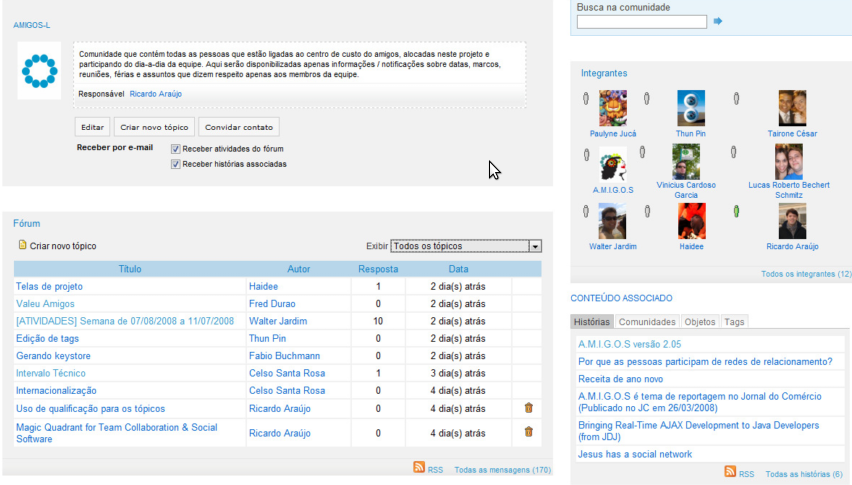
\includegraphics[width=0.7\textwidth]{imgs/screenshot-amigos.png}
  \caption{\emph{Screenshot} da interface do A.M.I.G.O.S.}
    \label{ap:fig:screenshot}
\end{figure}

Considerando os critérios estabelecidos no \chapref{ch:dominio}, temos que a
representação da rede precisa ser não-binária e envolver a maior quantidade de
dimensões da força do laço possível; Por esta razão focaremos nas interações
textuais do a.m.i.g.o.s. usando o conceito de atenção apresentado na
\secref{sec:teoria_atencao}. Para a análise de influência, seguindo a orientação
apresentada na \secref{sec:sobre-proem}, usaremos duas métricas, uma medial e
outra radial; ambas baseadas no volume dos caminhos. As escolhidas foram a
\emph{Flow betweenness} de \citeauthor{Freeman1991} e o poder de
\citeauthor{Bonacich1987}; as razões dessa escolha são a de que atendem aos
critérios de serem sensíveis tanto à estrutura macro da rede, quanto a
configuração local do nó, e também por simplicidade de implementação.

 

\section{Entendendo os Dados}
\label{ap:sec:dados}

Como para os fins desse estudo nos foi cedido o acesso a uma ``fotografia'' do
banco de dados do ambiente, então será uma análise intrínseca; não precisaremos
de \emph{crawlers}. Devido à complexidade de implementar algoritmos de análise de
sentimento, seguiremos uma abordagem ingênua e não consideraremos a intenção da
interação. Como se trata de interações em um contexto organizacional fechado, é
pouco provável que tenhamos disruptores e históricos longos de adversidade, de
forma que podemos considerar que muitas interações entre dois membros é uma bom
indicativo da positividade de suas intenções.

O poder da abordagem apresentada na \secref{sec:teoria_atencao} é a integração
de vários tipos de interação, conquanto sejam textuais. Então utilizaremos
quatro medianeiros textuais reconhecidos no ambiente e classificaremos de
acordo com a tipologia apresentada na \secref{sec:tipologia}:

\begin{description}
\item[Tópicos] são mensagens que \textbf{iniciam} discussões nos fóruns das
comunidades. A abrangência é individual desenvolvida, já que é direcionada aos
membros daquela comunidade apenas.
\item[Respostas] compõem o resto das mensagens nas discussões dos fóruns e
seguem naturalmente os tópicos e umas às outras. A abrangência também é
individual desenvolvida.
\item[Histórias] que são os textos de propósito geral que podem ser visualizados
por qualquer pessoa dentro do sistema, com algumas exceções. A abrangência,
nesse caso, pode ser individual desenvolvida quando relacionada a uma comunidade
apenas ou individual generalizada quando para todo o ambiente.
\item[Comentários] relativos às histórias publicadas. Cada história tem um
espaço público onde qualquer membro pode ler e publicar sua opinião, trata-se
portanto de uma interação de abrangência comum.
\end{description}

É importante denotar a abrangência de cada medianeiro pois que afeta diretamente
o cálculo da atenção residual que cada autor tem com seus leitores. Usaremos o
coeficiente $\beta$ igual ao inverso multiplicativo da quantidade de membros da
abrangência, assim cada autor cede parcelas iguais a sua audiência por cada
interação. Para interações de abrangência generalizada para todo o ambiente, como
é o caso da grande maioria das histórias cadastradas, temos que $\beta=0$, por
tanto, o autor não cede atenção residual para ninguém.

Como nossa anális é intrínseca, pela disposição da informação no banco de dados
podemos saber exatamente qual membro acessou e leu quais tópicos e histórias.
Por esta razão, definimos o coeficiente $\alpha$ da seguinte maneira: 0, caso
não tenha lido; $0.2$, caso tenha. Sendo assim, membros da abrangência que não
leram não cedem atenção ao autor, membros que leram cedem 20\% do total possível
e aqueles que leram e responderam ou comentaram cedem 100\% da atenção.

Fizemos $\gamma=^1/_2$ de forma que a atenção transitiva decai para a metade a
cada elo da \textit{thread}. Infelizmente, mesmo a análise sendo intrínseca, não
tivemos acesos a interações passivas do usuário como, por exemplo, o tempo que
ele passou em cada leitura ou logado no sistema. Dessa forma é complicado
estimar uma função de participação $E(.)$, porém nós podemos considerar o
próprio índice de atividade calculado pelo sistema como aproximação desse
parâmetro.

\section{Preparando os dados}
\label{ap:sec:preparacao}

Segundo \citet{Cios2005}, em torno de 45\% do esforço total empregado no
processo de mineração de dados é usado no passo de preparação dos dados, como
podemos ver na \figref{ap:fig:esforco}. Por esta razão produzimos como
subproduto dessa atividade um \emph{framework} enxuto para a extração e
manipulação dos dados. O banco original é acessível via \emph{SQL}, através do
qual extraímos as interações e armazenamos em outro banco com controle de data
de quando cada interação foi capturada; em cima desse banco criamos uma
estrutura que abstrai a camada de dados da aplicação, permitindo ao pesquisador
utilizar se concentrar na exploração do grafo.

\begin{figure}[h!]
  \centering
    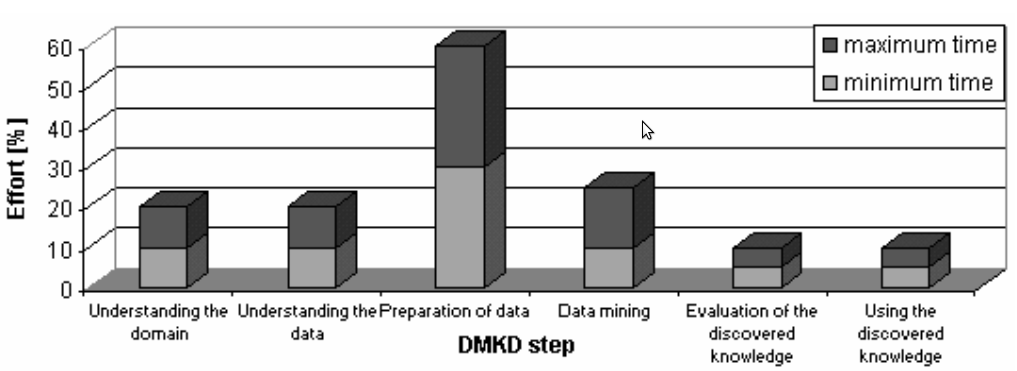
\includegraphics[width=0.7\textwidth]{imgs/preparation-time.png}
  \caption{Esforço relativo para cada passo do KDDM \citep{Cios2005}}
    \label{ap:fig:esforco}
\end{figure}

O \emph{framework} foi escrito em \emph{Python} e utiliza uma \emph{API} de
\emph{ORM} para esconder o serviço de banco de dados utilizado. Através dessa
modelagem o pesquisador tem simples acesso ao conjunto de membros da rede, ao
conjunto de suas interações (e propriedades) e a abrangência de cada. Nesse
quesito, precisamos separar o público-alvo esperado e o real (ver
\figref{ap:fig:grafo}), com isso, a atenção reflexiva é calculada em cima do
público-alvo esperado, enquanto que só o público-alvo direto cede atenção direta
para o autor. Com isso é possível que autores cedam mais do que recebem, à medida
que produzem para uma comunidade onde poucos ou nenhum de seus membros consomem
este conteúdo.

\begin{figure}[h!]
  \centering
    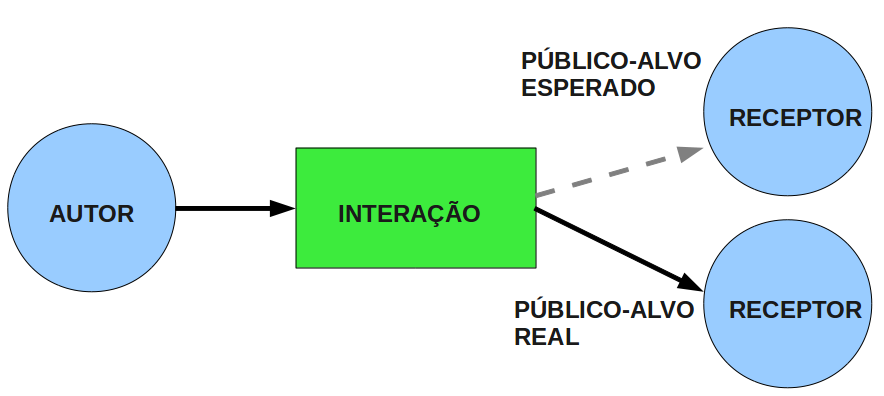
\includegraphics[width=0.7\textwidth]{imgs/naif-grafo.png}
  \caption{Exemplo de modelagem no \emph{framework}}
    \label{ap:fig:grafo}
\end{figure}

Implementamos o algoritmo de cálculo de atenção como apresentado na
\secref{sec:formalizacao}, e obtivemos o resultado separado para os dois grupos
de interações textuais: tópicos e resposta; histórias e comentários. O resultado
que encontramos é apresentado na \figref{ap:fig:cdf}, onde a distribuição da
carga de atenção parece seguir uma lei de potência. Essa característica é
interessante porque mimetiza a propriedade \emph{scale-free} das redes
sociais. 

As Figuras \ref{ap:fig:contatos}, \ref{ap:fig:topicos}, \ref{ap:fig:narrativas} e
\ref{ap:fig:completa} aprensentam visualizações das quatro redes concebidas: uma
não textual, que é a de contatos; três textuais, ou seja, utilizando nosso
algoritmo de atenção, sobre apenas tópicos e suas repostas, apenas histórias e
seus comentários e uma completa considerando tópicos e histórias. Na
\tabref{ap:tab:estatisticas} apresentamos algumas estatísticas sobre as quatro
redes, indicando grau médio de reciprocidade em todas as representações. Alto
grau de reciprocidade era esperado para as redes de atenção devido à atenção
residual, assim toda interação gera uma conexão da audiência para o autor e sua
recíproca do autor para a audiência, mesmo que em menor intensidade. O resultado
encontrado, principalmente na rede de tópicos, indica que apesar do autor da
mensagem visar obter a atenção de toda uma comunidade, poucos foram os que
efetivamente se prestaram a isso.

\begin{figure}[h!]
  \centering
    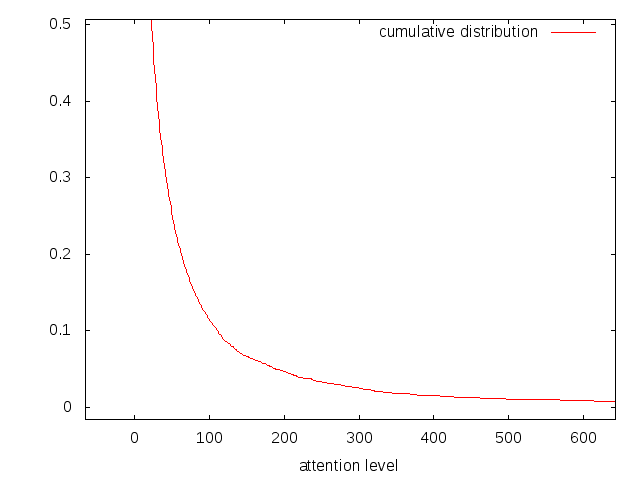
\includegraphics[width=0.7\textwidth]{imgs/cdf-final.png}
  \caption{Distribuição da Probabilidade Cumulativa da Atenção}
    \label{ap:fig:cdf}
\end{figure}

\begin{figure}[h!]
  \centering
    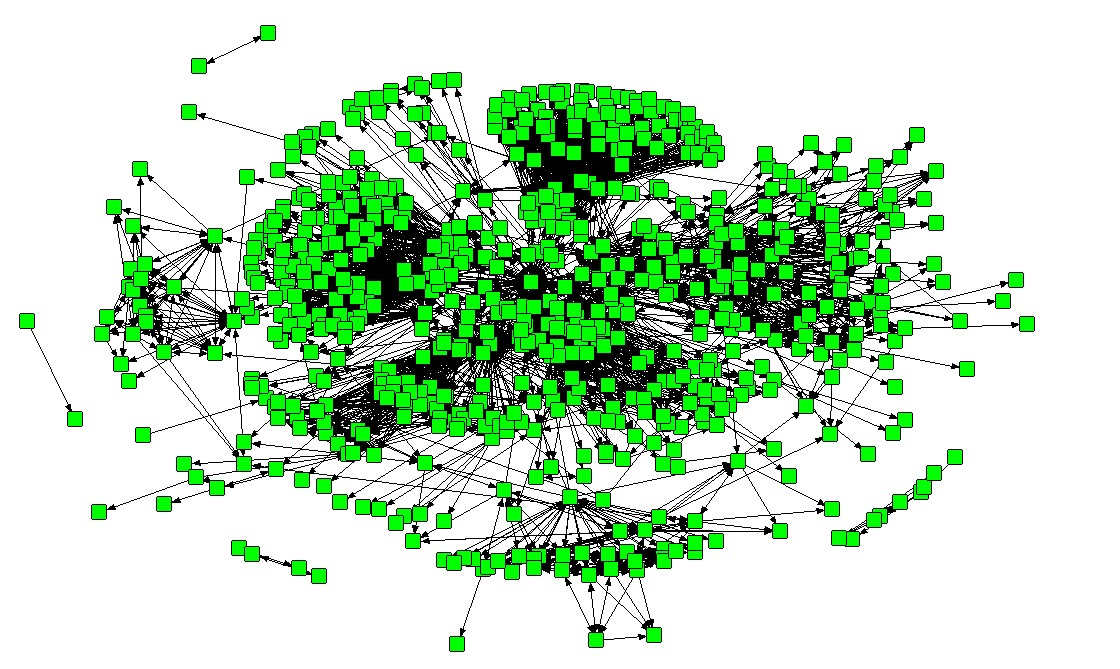
\includegraphics[width=0.7\textwidth]{imgs/contatos.jpg}
  \caption{Visualização da rede de contatos do a.m.i.g.o.s.}
    \label{ap:fig:contatos}
\end{figure}

\begin{figure}[h!]
  \centering
    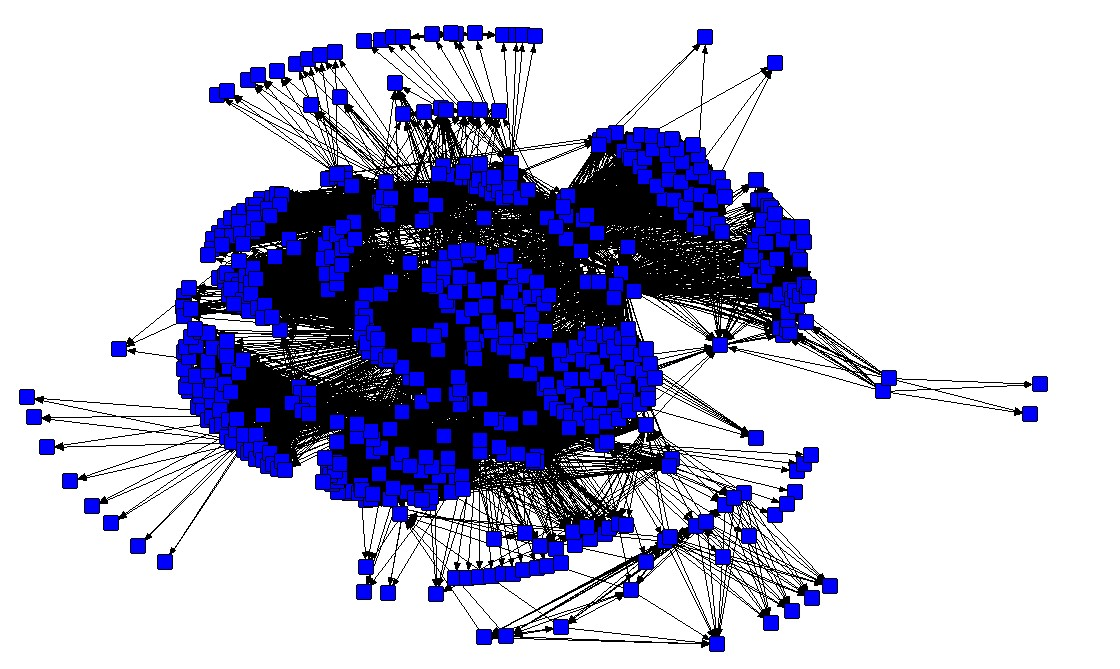
\includegraphics[width=0.7\textwidth]{imgs/topicos.jpg}
  \caption{Visualização da rede de tópicos do a.m.i.g.o.s.}
    \label{ap:fig:topicos}
\end{figure}

\begin{figure}[h!]
  \centering
    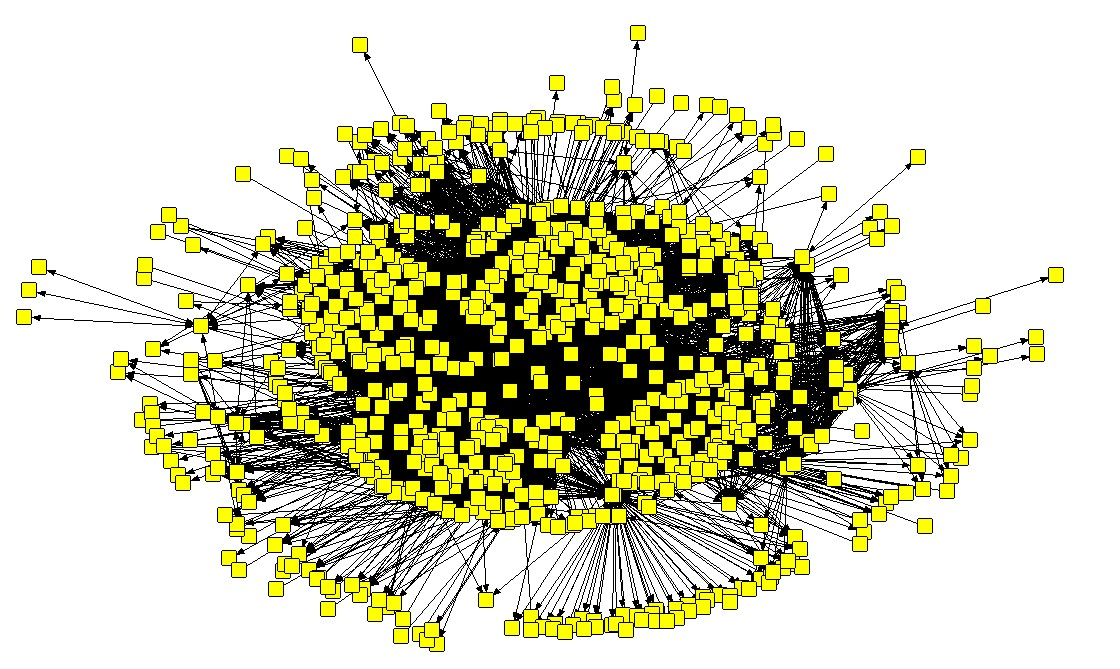
\includegraphics[width=0.7\textwidth]{imgs/narrativas.jpg}
  \caption{Visualização da rede de histórias do a.m.i.g.o.s.}
    \label{ap:fig:narrativas}
\end{figure}

\begin{figure}[h!]
  \centering
    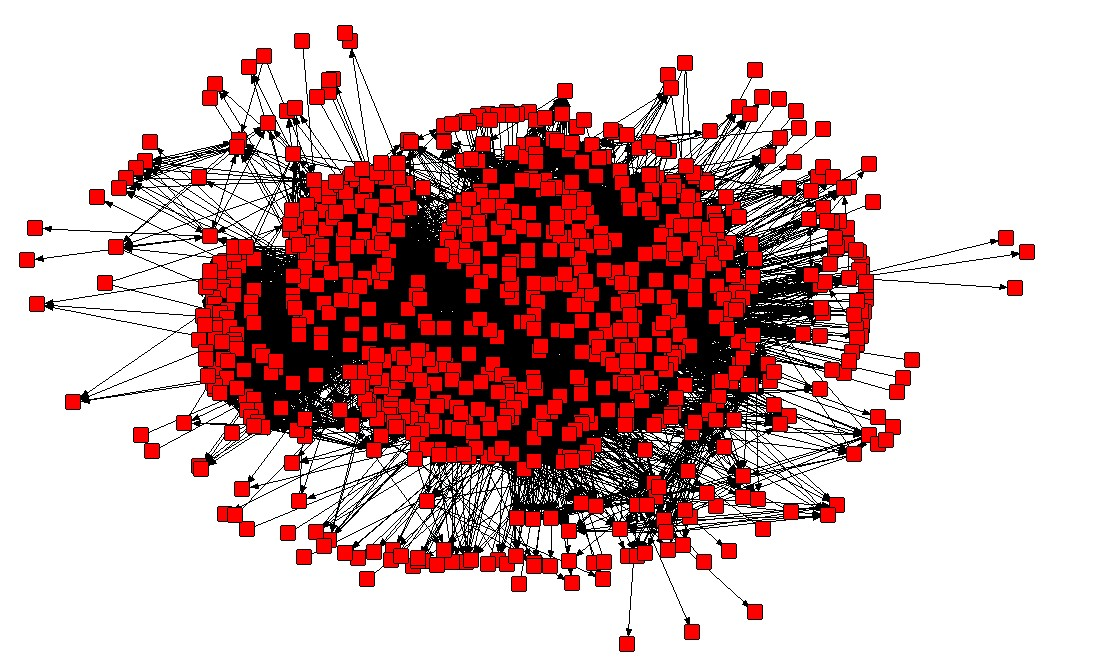
\includegraphics[width=0.7\textwidth]{imgs/completa.jpg}
  \caption{Visualização da rede de atenção completa do a.m.i.g.o.s.}
    \label{ap:fig:completa}
\end{figure}

\begin{table} [htbp]
	\large       % tamanho da fonte 
	\setlength{\arrayrulewidth}{2\arrayrulewidth}  % espessura da  linha
	\setlength{\belowcaptionskip}{10pt}  % espaço entre caption e tabela
	\caption{Tamanho e propriedades das redes} \centering   % tabela centralizada
	\begin{tabular}{| c | c | c | c | c |}
	\hline
	Rede & Tam. Componente & Densidade & Desv. Padrão & Reciprocidade \\ \hline
	Contatos & 680 & 0,01 & - & 0,55 \\
	Tópicos & 618 & 1,57 & 64,72 & 0,42\\
	Narrativa & 815 & 2,37 & 38,04 & 0,53\\
	Completa & 838 & 3,09 & 63,93 & 0,57\\ \hline
	\end{tabular}
	\label{ap:tab:estatisticas}
\end{table}

Antes de prosseguir com a análise da influência, podemos avaliar o quanto de
informação mútua existe nas redes mensuradas. Como foi mostrado na
\secref{sec:criterios}, redes com alto grau de sobreposição podem ser
descartadas uma em favor da outra para reduzir o conjunto a ser analisado na
próxima etapa. Na \tabref{ap:tab:qap} temos o resultado para as quatro redes
mensuradas. Se considerarmos separadamente tópicos e histórias, veremos que eles
tem pouca coisa em comum; mas a rede completa de atenção por sua vez é
fortemente correlacionada com ambas, sugerindo sua utilização no lugar das
primeiras. Também notamos uma leve para moderada correlação positiva entre a
rede de contatos e a de atenção, apesar de não estarem relacionadas diretamente.
Essa diferença entre as redes justificaria também uma forte diferença na análise
da influência?

\begin{table}[htbp]
	\large
	\setlength{\arrayrulewidth}{2\arrayrulewidth}
	\setlength{\belowcaptionskip}{10pt}
	\caption{\emph{QAP} aplicado as quatro redes (p. < 0,001)} \centering
	\begin{tabular}{|c | c  c  c  c |}
	\hline
	QAP corr & completa & contatos & histórias & tópicos \\ \hline
	completa & 1 & 0,22 & 0,67 & 0,82 \\
	contatos & 0,22 & 1 & 0,23 & 0,12 \\
	histórias & 0,67 & 0,23 & 1 & 0,13 \\
	tópicos	& 0,82 & 0,12 & 0,13 & 1 \\ \hline
	\end{tabular}
	\label{ap:tab:qap}
\end{table}


\section{Análise da influência}
\label{ap:sec:analise}

Após a mensuração das redes, apresentada na seção anterior, passamos à análise
de influência propriamente dita. Havíamos decidido usar o \emph{Flow
Betweenness} no passo 1 desse projeto, devido à natureza valorada da
representação, porém não nos foi possível alcançar nosso intento devido ao alto
custo computacional que se mostrou para essa métrica. Sendo assim, substituímos
pela métrica simples de \emph{Betweenness} que dicotomiza a rede pela média,
isto é, os laços cuja força seja maior ou igual que a média continuam (1) e os
abaixo são removidos (0). A métrica de \citeauthor{Bonacich1987} foi calculada
como planejada.

As Tabelas \ref{ap:tab:cent-contatos} e \ref{ap:tab:cent-completa} apresentam os
resultados para a métrica de \emph{Betweenness} nas rede de contatos e na de
atenção. No cabeçalho temos o índice de centralização de
\citeauthor{Freeman1979} que indica o quão próximo a rede está de um gráfico do
tipo estrela. É interessante notar que a rede de atenção formada apenas com os
tópicos e suas resposta apresentou o maior grau de centralização: 37,18\%;
enquanto que as histórias apresentaram: 24,20\%. Destacamos em negrito os
membros que se repetiram nas quatro representações: contatos, tópicos, histórias
e completa. É interessante notar que apesar não haver nenhuma relação direta
entre a rede completa e a de contatos, aquela manteve quase que inalterada a
ordenação do grupo que intersecta ambas.

\begin{table}[htbp]
	\large       % tamanho da fonte 
	\setlength{\arrayrulewidth}{2\arrayrulewidth}  % espessura da  linha
	\setlength{\belowcaptionskip}{10pt}  % espaço entre caption e tabela
	\caption{Os 9 membros mais bem posicionados na rede de Contatos} \centering   
	\begin{tabular}{| c | c |}
	\hline
	Contatos & Centralização=30,81\% \\ \hline\hline
	Membro & \emph{Betweenness} \\ \hline
	\textbf{3} & \textbf{31,06} \\
	\textbf{8} & \textbf{13,48} \\
	135 & 11,44 \\
	\textbf{2} & \textbf{8,68} \\
	\textbf{200} & \textbf{5,14} \\
	201 & 4,84 \\
	\textbf{796} & \textbf{4,82} \\
	601 & 4,57 \\
	665 & 4,55 \\ \hline
	\end{tabular}
	\label{ap:tab:cent-contatos}
\end{table}

\begin{table}[htbp]
	\large       % tamanho da fonte 
	\setlength{\arrayrulewidth}{2\arrayrulewidth}  % espessura da  linha
	\setlength{\belowcaptionskip}{10pt}  % espaço entre caption e tabela
	\caption{Os 9 membros mais bem posicionados na rede de Atenção} \centering   
	\begin{tabular}{| c | c |}
	\hline
	Completa & Centralização=23,07\% \\ \hline\hline
	Membro & \emph{Betweenness} \\ \hline
	\textbf{3} & \textbf{23,18} \\
	\textbf{2} & \textbf{12,53} \\
	\textbf{8} & \textbf{8,99} \\
	\textbf{200} & \textbf{3,65} \\
	\textbf{796} & \textbf{3,37} \\
	6 & 1,79 \\
	665 & 1,7 \\
	397 & 1,61 \\
	201 & 1,5 \\\hline
	\end{tabular}
	\label{ap:tab:cent-completa}
\end{table}

Quando analisamos a correlação entre os resultados de centralidade das quatro
redes mensuradas, apresentada na \tabref{ap:tab:cent-corr}, podemos perceber o
impacto da decisão em usar a métrica de \emph{Betweenness} no lugar da original.
A dicotomização da rede quase que totalmente mimetiza o padrão de posicionamento
encontrado na rede de contatos; i.e., removido o peso dos laços, parece-nos que
os atores fazem as mesmas escolhas em termos de quem interagir e de quem
adicionar aos seus contatos. Entretando, o índice de \citeauthor{Bonacich1987}
leva em consideração este peso para a rede de atenção, logo seus resultados
devem se diferenciar bastante da rede não-textual.

\begin{table}[htbp]
	\large       % tamanho da fonte 
	\setlength{\arrayrulewidth}{2\arrayrulewidth}  % espessura da  linha
	\setlength{\belowcaptionskip}{10pt}  % espaço entre caption e tabela
	\caption{Correlação do índice de centralidade} \centering   
	\begin{tabular}{| c | c c c c|}
	\hline
	\emph{Betweenness} & completa & contatos & histórias & tópicos \\ \hline
	completa & 1 & 0,89 & 0,96 & 0,94 \\
	contatos & 0,89 & 1 & 0,91 & 0,87 \\
	histórias & 0,96 & 0,91 & 1 & 0,93 \\
	tópicos & 0,94 & 0,87 & 0,93 & 1 \\\hline
	\end{tabular}
	\label{ap:tab:cent-corr}
\end{table}

Para o índice de prestígio, temos grande disparidade nos resultados apresentados
pelas redes textuais e não-textuais, como era de se esperar. As Tabelas
\ref{ap:tab:prest-contato} e \ref{ap:tab:prest-completa} nos traz os melhores
colocados no índice de \citeauthor{Bonacich1987} para as redes de contatos e de
atenção respectivamente. Da mesma forma como nas de centralidade, os membros que
se repetiram nas melhores colocações em todas as quatro redes foram marcados em
negrito; neste caso, houve apenas um. Esse resultado nos diz que apesar de
estruturalmente a rede de atenção ser similar a de contatos, quando levamos em
consideração a intensidade dessas interações, a distribuição desigual da atenção
nos revela os influenciadores realmente ativos.

\begin{table}[htbp]
	\large       % tamanho da fonte 
	\setlength{\arrayrulewidth}{2\arrayrulewidth}  % espessura da  linha
	\setlength{\belowcaptionskip}{10pt}  % espaço entre caption e tabela
	\caption{Os 9 membros mais prestigiados na rede de Contatos} \centering   
	\begin{tabular}{| c | c |}
	\hline
	\citeauthor{Bonacich1987} & Contatos\\ \hline\hline
	Membro & \emph{Power} \\ \hline
	8 & 240,311 \\
	\textbf{3} & \textbf{189,279} \\
	397 & 128,291 \\
	385 & 120,024 \\
	419 & 119,683 \\
 	481 & 109,363 \\
 	422 & 108,501 \\
 	436 & 106,941 \\ 
 	452 & 106,314 \\\hline
	\end{tabular}
	\label{ap:tab:prest-contato}
\end{table}

\begin{table}[htbp]
	\large       % tamanho da fonte 
	\setlength{\arrayrulewidth}{2\arrayrulewidth}  % espessura da  linha
	\setlength{\belowcaptionskip}{10pt}  % espaço entre caption e tabela
	\caption{Os 9 membros mais prestigiados na rede de Atenção} \centering   
	\begin{tabular}{| c | c |}
	\hline
	\citeauthor{Bonacich1987} & Atenção\\ \hline\hline
	Membro & \emph{Power} \\ \hline
	2 & 649,7 \\
	665 & 304,450 \\
	681 & 264,112 \\
	711 & 205,687 \\
	668 & 132,357 \\
	\textbf{3} & \textbf{108,871} \\
	201 & 104,042 \\
	781 & 79,441 \\
	826 & 76,397 \\\hline
	\end{tabular}
	\label{ap:tab:prest-completa}
\end{table}

Como era de se esperar, não poderíamos ter muita compatibilidade entre o
resultado de contatos e o de atenção. A \tabref{ap:tab:prest-corr} nos confirma
isso, mas também nos indica que a quase totalidade (98\%) do prestígio advém
das interações nos fóruns (tópicos e respostas). Certamente também
encontraríamos essa diferença na centralidade se não tivessemos dicotomizado os
dados.

\begin{table}[htbp]
	\large       % tamanho da fonte 
	\setlength{\arrayrulewidth}{2\arrayrulewidth}  % espessura da  linha
	\setlength{\belowcaptionskip}{10pt}  % espaço entre caption e tabela
	\caption{Correlação do índice de prestígio} \centering   
	\begin{tabular}{| c | c c c c|}
	\hline
	\emph{Betweenness} & completa & contatos & histórias & tópicos \\ \hline
	completa & 1 & 0,07 & 0,1 & 0,98 \\
	contatos & 0,07 & 1 & 0,28 & 0,06 \\
	histórias & 0,1 & 0,28 & 1 & 0,06 \\
	tópicos & 0,98 & 0,06 & 0,06 & 1 \\\hline
	\end{tabular}
	\label{ap:tab:prest-corr}
\end{table}

Finalmente, avaliamos a utilidade das métricas calculadas tendo por base o que
foi apresentado na \secref{sec:rel_proe}. Sendo assim, caso a rede mensurada
não tenha propriedades estruturais de uma comunidade de prática, então a métrica
radial que escolhemos, o poder de \citeauthor{Bonacich1987}, terá pouca
utilidade prática já que os \emph{hubs} estarão isolados em seus
\emph{clusters}. A \tabref{ap:tab:comu_prat} nos mostra que esse não é o caso,
encontramos um alto grau de coesão e padrão núcleo/periferia nas redes
mensuradas. Sendo a rede de tópicos a que mais se destacou com esse padrão,
talvez por representar o dia a dia dos colaboradores em suas trocas de
mensagens.

\begin{table}[htbp]
	\large       % tamanho da fonte 
	\setlength{\arrayrulewidth}{2\arrayrulewidth}  % espessura da  linha
	\setlength{\belowcaptionskip}{10pt}  % espaço entre caption e tabela
	\caption{Indícios de comunidades de prática} \centering   
	\begin{tabular}{| c | c | c | c | c |}
	\hline
	 & completa & contatos & histórias & tópicos \\ \hline
	Coeficiente Clusterização & 0,68 & 0,55 & 0,66 & 0,74 \\
	Coef. Cluster. Ponderado & 0,5 & 0,26 & 0,5 & 0,4 \\
	Distância média & 2,84 & 3,82 & 2,64 & 1,72 \\
	Adequação Núcleo/Perif. & 0,52 & 0,02 & 0,38 & 0,62 \\\hline
	\end{tabular}
	\label{ap:tab:comu_prat}
\end{table}

Para ilustrar a aplicação desse novo conhecimento adquirido, vamos utilizar uma
quinta e ultima mensuração do a.m.i.g.o.s.: a rede de recomendação. A rede de
atenção se comporta de certa forma às avessas, se um laço vai de $a$ para $b$ é
por que houve uma interação de $b$ para $a$. Então temos que prestígio, na rede
atenção, é sinônimo de atividade; Usuários ativos que publicam muito conteúdo
recebem muita atenção e por isso possuem alto prestígio. Para testar essa
afirmação, mensuramos uma rede binária direcionada ingênua a partir das
recomendações encontradas no sistema. Nessa representação, se $X_{ab}=1$ então
$a$ enviou uma recomendação de algo (comunidade, tópico ou história) para $b$.
Só pra constar, recomendações são interações de conteúdo não-textual e de
abrangência individual básica (i.e., de membro a membro), no geral, sua
intenção é informativa ou conectiva.

\begin{figure}[h!]
  \centering
    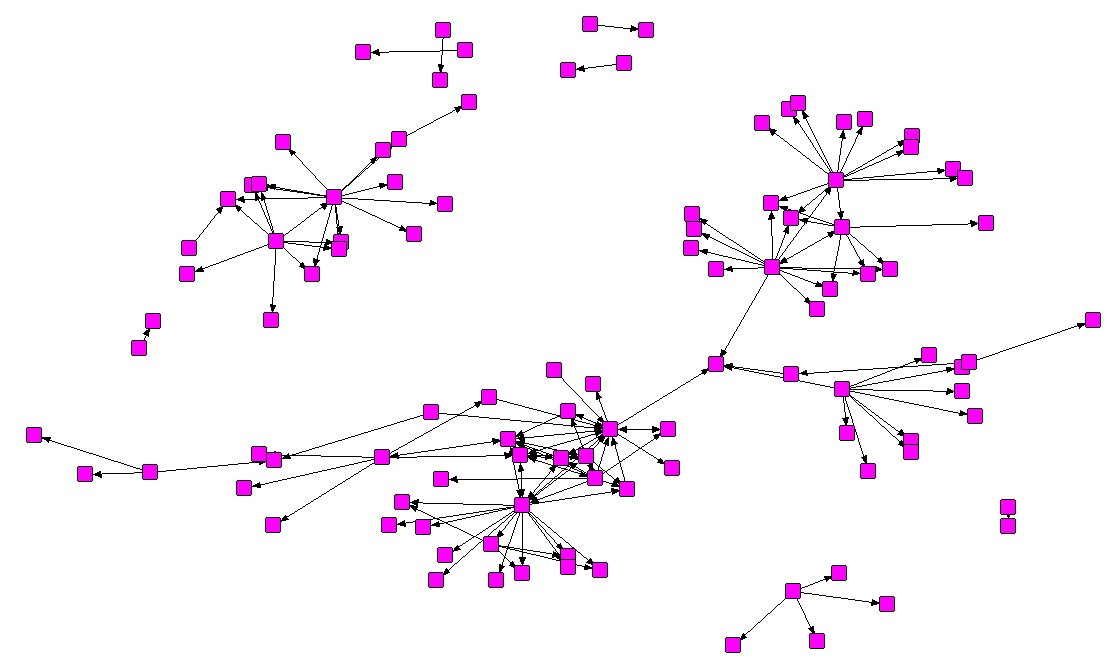
\includegraphics[width=0.7\textwidth]{imgs/recmd.jpg}
  \caption{Visualização da rede de recomendação do a.m.i.g.o.s.}
    \label{ap:fig:recmd}
\end{figure}

Para o caso de uma rede como a da \figref{ap:fig:recmd}, temos que os atores
mais centrais são também os mais ativos, por que recomendam algo aos outros.
Neste caso em particular, como foram poucas recomendações registradas no sistema
até o momento em que nos foi fornecido o acesso, calculamos apenas 10 atores com
alguma centralidade. Se o prestígio em nossa rede de atenção mede realmente a
intensidade que um membro atua no ambiente, então é de se esperar que
encontremos uma forte interseção entre esses dois conjuntos (prestígio na rede
de atenção e centralidade na rede de recomendação).

É exatamente o que encontramos, os 5 membros mais centrais nas recomendações já
aparecem na lista dos 10 mais em prestígio. Encontramos até o 9 na  lista dos 100
mais e o último colocado nas recomendações ocupa o 210\textordmasculine~lugar
na de prestígio. Quanto a ordenação, encontramos uma correlação espantosa entre os
dois atributos: 0,929. O que indica que com muita pouca variação, quem tem mais
prestígio também recomendou mais.

E no caso da centralidade para redes de atenção, o que representa? No nosso
caso, pouco devido à dicotomização da rede que mascarou a diferença entre
autores e receptores. Entretanto, considerando o uso da \emph{Flow Betweenness}
original, o esperado é que os atores centrais fossem aqueles com muitas ligações
fortes entre vários atores, isto quer dizer que são membros receptores que se
posicionam na rede consumindo informação de fontes variadas. Esses receptores
atuam então como \emph{brokers} repassando as informações que acham válidas. 

Em uma utilização do resultado desse exercício para o marketing ou a simples
divulgação de informação, deveriamos visar primeiro os de alto prestígio, esses
serão aqueles onde a cascata começará, mas também não devemos esquecer dos de
alta centralidade. Se no propagar da cascata a novidade encontrar um
\emph{broker} já inclinado a aceitar, a probabilidade vai ser muito maior da
onda se espalhar em novos ambientes.

\section{Resultados encontrados}
\label{ap:sec:resultados}

Em primeiro lugar, o resultado positivo encontrado nos dados para as hipóteses
levantadas no começo do processo, sugere que o método de mineração de dados
serviu seu propósito de orientar a pesquisa com segurança. A tipologia de
interações e o \emph{framework} conceitual que descrevemos no decorrer desse
trabalho, aplicaram-se adequadamente ao estudo de caso. Não obstante disso
deduza-se necessariamente sua aplicabilidade a outros tipos de casos,
acreditamos que ele foi definido geral o suficiente para tal.

Inesperadamente, talvez por necessidade, também iniciamos a construção de uma
ferramenta simples para o auxílio na preparação dos dados. Em uma busca rápida ao
site da \emph{Internacional Network for Social Network Analysis}
\citep{INSNA2010} encontramos de um total de 29 \emph{softwares} catalogados para
o uso em SNA, desses observamos: 11 são para visualização da rede, 5 são pacotes
estatísticos e matemáticos, 2 são de transformação de dados (XML e áudio), 8 são
voltados para algoritmos de SNA propriamente, como o UCINET \citep{Borgatti2010}
que foi usado para calcular as métricas nesse estudo de caso) e 3 envolvem a
extração dos dados propriamente dita. Desses últimos, o que mais se aproxima da
ferramenta desenvolvida nesse projeto é o UrlNet \citep{Hunscher2010} que
facilita a criação de \emph{crawlers} para a \emph{web}; curiosamente também
desenvolvido na linguagem Python. Mesmo assim, acreditamos que há espaço para a
nossa ferramenta, pois é de propósito geral e permite reunir o resultados dos
\emph{crawlers} em modelos: membros x interação.

 

